\documentclass{beamer}
\usepackage{listings}
\usepackage{blkarray}
\usepackage{listings}
\usepackage{subcaption}
\usepackage{url}
\usepackage{tikz}
\usepackage{tkz-euclide} % loads  TikZ and tkz-base
%\usetkzobj{all}
\usetikzlibrary{calc,math}
\usepackage{float}
\newcommand\norm[1]{\left\lVert#1\right\rVert}
\renewcommand{\vec}[1]{\mathbf{#1}}
\usepackage[export]{adjustbox}
\usepackage[utf8]{inputenc}
\usepackage{amsmath}
\usepackage{amsfonts}
\usepackage{tikz}
\usepackage{hyperref}
\usepackage{multirow}
\usepackage{bm}
\hypersetup{
    colorlinks = true,
    linkbordercolor = {white},
    linkcolor={red},
    citecolor={green},
    filecolor={blue},
	menucolor={red},
	runcolor={cyan},
	urlcolor={blue},
	breaklinks=true
}
\usetikzlibrary{automata, positioning}
\usetheme{Boadilla}
\providecommand{\pr}[1]{\ensuremath{\Pr\left(#1\right)}}
\providecommand{\mbf}{\mathbf}
\providecommand{\qfunc}[1]{\ensuremath{Q\left(#1\right)}}
\providecommand{\sbrak}[1]{\ensuremath{{}\left[#1\right]}}
\providecommand{\lsbrak}[1]{\ensuremath{{}\left[#1\right.}}
\providecommand{\rsbrak}[1]{\ensuremath{{}\left.#1\right]}}
\providecommand{\brak}[1]{\ensuremath{\left(#1\right)}}
\providecommand{\lbrak}[1]{\ensuremath{\left(#1\right.}}
\providecommand{\rbrak}[1]{\ensuremath{\left.#1\right)}}
\providecommand{\cbrak}[1]{\ensuremath{\left\{#1\right\}}}
\providecommand{\lcbrak}[1]{\ensuremath{\left\{#1\right.}}
\providecommand{\rcbrak}[1]{\ensuremath{\left.#1\right\}}}
\providecommand{\abs}[1]{\vert#1\vert}
\newcommand*{\permcomb}[4][0mu]{{{}^{#3}\mkern#1#2_{#4}}}
\newcommand*{\perm}[1][-3mu]{\permcomb[#1]{P}}
\newcommand*{\comb}[1][-1mu]{\permcomb[#1]{C}}

\newcounter{saveenumi}
\newcommand{\seti}{\setcounter{saveenumi}{\value{enumi}}}
\newcommand{\conti}{\setcounter{enumi}{\value{saveenumi}}}

\makeatletter
\newenvironment<>{proofs}[1][\proofname]{%
    \par
    \def\insertproofname{#1\@addpunct{.}}%
    \usebeamertemplate{proof begin}#2}
  {\usebeamertemplate{proof end}}
\makeatother
%% Theme choice:
%\usetheme{CambridgeUS}

% Title page details: 
\title{A Simple Problem On Binomial Distribution} 
\author{Chittepu Rutheesh Reddy\\
 CS21BTECH11014}
\date{\today}
\logo{\large \LaTeX{}}


\begin{document}

% Title page frame
\begin{frame}
    \titlepage 
\end{frame}

% Remove logo from the next slides
\logo{}


% Outline frame
\begin{frame}{Outline}
    \tableofcontents
\end{frame}




% Lists frame
\section{Question}
\begin{frame}{Question}

\begin{block}
{\textbf{Q15 [12$^{th}$ CBSE Probability Exercise 13.5]:}}

The probability that a student is not a swimmer is $\frac{1}{5}$. Then
the probability that out of five students, four are swimmers is?

\end{block}
\end{frame}


% Blocks frame
\section{Solution}

\begin{frame}{Solution}
Let X be the number of students and given that the probability of a student being swimmer is $\frac{1}{5}$

Then $X$ has the binomial distribution  
\begin{align}
\pr{X=k} = \comb{n}{k}p^k\brak{1-p}^{n-k}
\end{align}
 Here,  
 \begin{align}
 p=\frac{1}{5}\\
 n=5\\
 k=4
 \end{align}
$\therefore$ The required probability is $\comb{5}{4}\brak{\frac{4}{5}}^4\brak{\frac{1}{5}}$
\end{frame} 

\begin{frame}{Solution}

 \begin{figure}[h!]  
  \graphicspath{{./figs/}}  
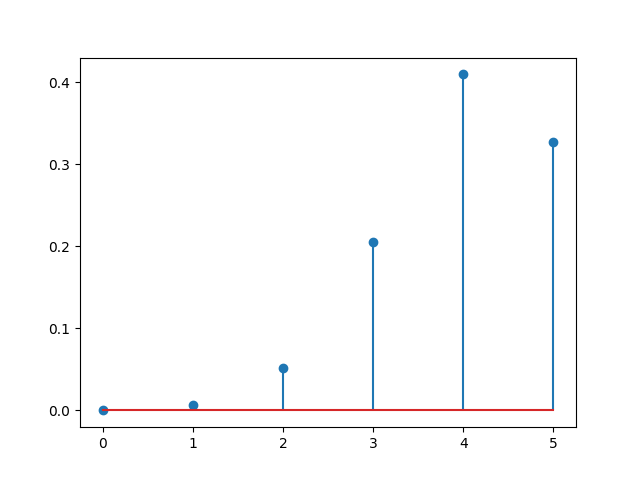
\includegraphics[scale=0.6]{Figure_1}
\label{Fig1}
\caption{pmf of this distribution}

\end{figure}

\end{frame}

\begin{frame}{Solution}

 \begin{figure}[h!]  
  \graphicspath{{./figs/}}  
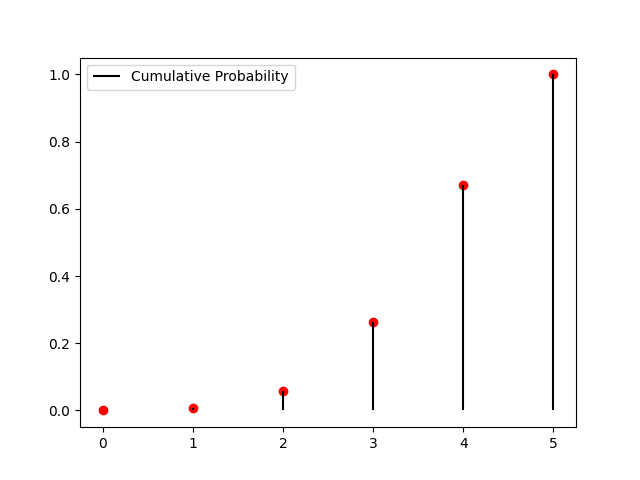
\includegraphics[scale=0.6]{Figure_2}
\label{Fig1}
\caption{cdf of this distribution}

\end{figure}

\end{frame}
\end{document}